\documentclass[12pt]{article}
\usepackage{hyperref}
\usepackage{amsmath, amssymb, amsfonts}
\usepackage[margin=2cm]{geometry}
\usepackage{xcolor}
\usepackage{graphicx}
\usepackage{xparse}
\usepackage{enumitem}
\parindent 0px
\newcommand{\W}{\(\Omega\)}
\newcommand{\w}{\(\omega\)}
\newcommand{\lb}{\left|\rightarrow\right.}
\newcommand{\enter}{\textcolor{white}{1}}\ExplSyntaxOn
\newcommand{\sub}[1]{\textsubscript{#1}}
\newcommand{\super}[1]{\textsuperscript{#1}}

\NewDocumentCommand{\bo}{m}
 {
   \bold_commas:n { #1 }
 }

\cs_new:Npn \bold_commas:n #1
 {
   \seq_set_split:Nnn \l_tmpa_seq { , } { #1 }
   \seq_map_indexed_function:NN \l_tmpa_seq \__bold_commas_aux:nn
 }

\cs_new:Npn \__bold_commas_aux:nn #1 #2
 {
   \textbf{#2}
   \int_compare:nNnTF { #1 } < { \seq_count:N \l_tmpa_seq }
     { , }
     { }
 }

\ExplSyntaxOff

\title{Operating System}
\author{Me lol}
\date{\today}

\begin{document}
\maketitle
\vspace{13cm}
\begin{large}\textbf{Notes}\end{large}
\begin{itemize}
\item PYQs of BEI's CT612, BCT's CT656, BCT's EX652 and BCT's EG682CT are combined.
\item BEI's CT612 questions' markings are \texttt{stylized with this font for clarity}.
\item The marking of questions of 66 Magh is \bo{not} \bo{given}. All marking given in this collection are \bo{assumed} marks based on other pyq's. 
\end{itemize}
\pagebreak
\tableofcontents
\pagebreak

\section{Introduction}
\begin{center}(5 Hours/10 Marks)\end{center}
\subsection{Operating System and Function}
\begin{enumerate}
\item Define operating system.\hfill[1] \begin{footnotesize}(\bo{\texttt{80 Bh}, 80 Ch, 79 Ch, 76 Bh}, 76 Ba, 75 Ba, \bo{72 Ash}, 71 Ma, 65 Ka)\end{footnotesize}
\item Explain the functions of Operating System.\hfill[3] \begin{footnotesize}(\bo{76 Bh}, 75 Ba, 73 Ma, \bo{68 Bh})\end{footnotesize} [4] \begin{footnotesize}(\bo{72 Ash})\end{footnotesize} \\
$\lb$What are the primary purposes of an operating system? Explain.\hfill[3] (\bo{73 Bh})
\item How does operating system provide a beautiful interface to user?\hfill[3] (\bo{\texttt{81 Bh}})
\item Justify how OS act as resource manager.\hfill[3]\begin{small} (\texttt{81 Ba}, \bo{77 Ch}, 76 Ba)\end{small} [4]\begin{small} (68 Ma, 65 Ka)\end{small}
\item Explain the statement: Operating system acts as a broker between hardware and application program.\hfill[4] (\bo{\texttt{80 Bh}, 79 Ch})
\item Explain OS as an Extended Machine.\hfill[2] (\texttt{80 Ba}, 70 Ma)\\
$\lb$ How does an OS create abstraction? Explain with reference to OS as an extended machine.\hfill[5] (\bo{69 Bh})
\item Explain the virtual machine structure. What are the benefits over other operating system architecture?\hfill[2+2] (\bo{74 Bh, 72 Ash})
\item Why Operating system is termed as virtual machine?\hfill[2] (73 Ma)\\
$\lb$Explain operating system as a virtual machine.\hfill[2] (\bo{67 Mng}) [4] (\texttt{80 Ba})

\item Why should the operating system prevent users from accessing the boot sector?\hfill[2] (\bo{73 Bh})
\item Explain in detail about context switching.\hfill[4] (\bo{67 Mng})
\item What features does an operating system expose on top of the hardware to enhance user experience? Explain. \hfill[8] (\bo{66 Ma})
\end{enumerate}
\subsection{Evolution of Operating System}
\begin{enumerate}
\item Why operating system evolve over long periods of time?\hfill[1] (\texttt{81 Ba})
\end{enumerate}
\subsection{Type of Operating System: Batch, Interactive, Multiprocessing, Time Sharing and Real Time System}
\begin{enumerate}
\item Explain in brief any four types of OS.\hfill[5] (\bo{73 Bh})\\
$\lb$Briefly mention the type of operating system.\hfill[4] (71 Ma)
\item List the essential properties for the Batch-oriented and Interactive operating system.\\
\enter\hfill[4] (\bo{70 Bh})
\item Write down the major differences between following types of operating system.\\
\enter\hfill[8] (\bo{78 Ch, 71 Bh})\\
a. Batch system\hspace{7mm}b. Interactive system\hspace{7mm}c. Real time system\hspace{7mm}d. Time sharing system
\item Discuss the properties of batch system and real time system.\hfill[4] (76 Ba)
\item Explain multiprogramming, multiprocessing and distributed operating system.\hfill[6] (74 Bh)
\item For each of the following application which system (Batch or Interactive) is more suitable?\\
a. Word Processing \hspace{5cm}b. A flight simulator\hfill[6] (\bo{70 Bh})\\
c. Computing pi to million decimal places\hspace{9mm} d. Generating monthly bank statements\\ 
e. Generating mark statement by University \hspace{7mm}f. Data acquisition from temperature sensor
\end{enumerate}
\subsection{Operating System Components}
\begin{enumerate}
\item What do you understand by firmware? Can you relate with operating system? Are there any linkages among hardware, software, firmware and operating system?\hfill[10] (70 Ma)
\end{enumerate}
\subsection{Operating System Structure: Monolithic, Layered, Micro-Kernel, Client-Server, Virtual Machine}
\begin{enumerate}
\item What are the different structures of an operating system?\hfill[2] (\bo{67 Mng})
\item Why Exo-Kernel doesn't require Re-mapping of resources?\hfill[2] \begin{small}(\bo{\texttt{81 Bh}, 79 Ch})\end{small} [3] \begin{small}(\bo{80 Ch})\end{small}
\item Is layered structure of operating system is better than monolithic structure? Explain.\\
\enter \hfill[3] \begin{small}(\bo{\texttt{81 Bh}, 79 Ch})\end{small} [4] \begin{small}(\bo{80 Ch})\end{small} [10] \begin{small}(72 Ma)\end{small}
\item Differentiate between Monolithic Kernel and Micro-Kernel.\hfill[4] (\texttt{80 Ba}) [5] (71 Ma)
\item Distinguish between kernel and micro-kernel.\hfill[3] (70 Ma)
\item Explain about microkernel.\hfill[5] (\bo{68 Bh})
\item Explain the Monolithic and layered architecture of operating system. Explain which architecture is better among them and why?\hspace{6.7cm}[2+1] (\bo{76 Bh})\\
$\lb$Explain in brief about monolithic architecture and virtual machine.\hfill[3] (73 Ma)
\item Discuss about Microkernel and Monolithic structuring with their adv and disadv.[3] (\bo{77 Ch}) 
\item Why is the process table needed in a timesharing system? Is it also needed in personal computer systems running UNIX or Windows with a single user?\hfill[6] (\bo{\texttt{79 Bh}})
\item Distinguish between Shell and Kernel.\hfill[4] (\bo{\texttt{79 Bh}})
\end{enumerate}
\subsection{Operating System Services}
\subsubsection{System calls}
\begin{enumerate}
\item What is system call in OS?\hfill[1] \begin{small}(\bo{77 Ch, 76 Bh}, 75 Ba)\end{small} [2] \begin{small}(73 Ma)\end{small}
\item What is the purpose of a system call in an operating system?\\
\enter\hfill[2] \begin{small}(\bo{78 Ch, 71 Bh})\end{small} [3] \begin{small}(\bo{80 Ch}, 70 Ma)\end{small}
\item Define system call and explain its working mechanism with suitable example.\hfill[5] (\bo{69 Bh})
\item Illustrate the execution of system call read() to read a file.\hfill[5] (75 Ba)
\end{enumerate}
\subsubsection{Shell commands}
\begin{enumerate}
\item What do you mean by Shell?\hfill[1] (\bo{77 Ch})
\item What is pipe and shell?\hfill[4] (68 Ma)
\end{enumerate}
\subsubsection{Shell programming}
\begin{enumerate}
\item Write short notes on Shell Programming.\hfill[4] (\bo{75 Bh})
\end{enumerate}

\pagebreak
\section{Process Management}
\begin{center}(6 Hours/10 Marks)\end{center}
\subsection{Introduction to Process }
\begin{enumerate}[noitemsep, topsep = 0pt]
	\item Define process in OS and explain possible states. \hfill [2] (\bo{75 Bh})
\end{enumerate}
\subsubsection{Process description}
\begin{enumerate}
	\item What is priority of a process? Why do we need it? Explain. \hfill [2] (\bo{\texttt{80 Bh}})
\end{enumerate}
\subsubsection{Process states}
\subsubsection{Process control}
\begin{enumerate}[noitemsep, topsep = 0pt]
	\item Explain fork() and spawn() system calls in the OS. \hfill [3] (\texttt{81 Ba})
	
	\item Explain Context Switching with an example. \hfill [2] (\texttt{80 Ch})
	
	\item What information does a process control block contain? \hfill [3] (\bo{79 Ch})
\end{enumerate}
\subsection{Threads}
\subsection{Processes and Threads}
\begin{enumerate}[noitemsep, topsep = 0pt]
	\item Define Process and Threads. \hfill [2] (\bo{76 Bh})
	
	\item Write the difference between thread and process. \hfill [1] (\bo{77 Ch}) [2] (\bo{79 Ch}, 76 Ba)
	
	\item Why threads are called light weight process? \hfill [2] (\bo{\texttt{81 Bh}})
	
	\item What is multithreading? Explain five state process model with figure. \hfill [4] (\texttt{80 Ba})
	
	\item State 5-State process model. \hfill [2] (\bo{78 Ch})
	
	\item What are the advantages and disadvantages of implementing threads in user space?\\
	\enter \hfill [4] (\bo{\texttt{79 Ch}})
	
	\item Explain how multi threading provide better solution than single threading solution.\\
	\enter \hfill [3] (\bo{77 Ch})
\end{enumerate}
\subsection{Scheduling}
\subsubsection{Types of scheduling}
\begin{enumerate}[noitemsep, topsep = 0pt]
	\item Differentiate between Preemptive and Non-Preemptive Scheduling. \hfill [2] (\texttt{80 Ba})
\end{enumerate}
\subsubsection{Scheduling in batch system}
\subsubsection{Scheduling in Interactive System}
\subsubsection{Scheduling in Real Time System}
\subsubsection{Thread Scheduling}
\subsubsection{Numericals}
\begin{enumerate}
	\item Consider the following set of processes, with length of the CPU burst time given in milliseconds. \hfill [8] (\bo{\texttt{81 Bh}, 77 Ch})\\
	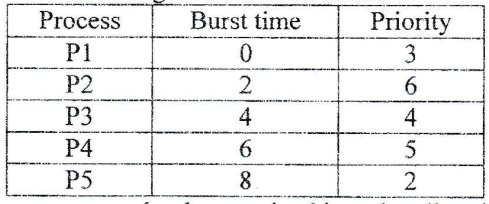
\includegraphics[width=3.5in]{os_1}\\
	A. All the processes are assumed to have arrived in order all at time 0.
	\begin{enumerate}[noitemsep, topsep = 0pt, label = \alph*.]
		\item Draw Gantt Chart Using FCFS, SJF scheduling algorithm.
		\item Find average turnaround time for each scheduling algorithm.
	\end{enumerate}
	B. Draw Gantt chart illustrating RR (quantum = 2) and highest ratio next (HRN) scheduling. Also find average waiting and average turn around time for each of the algorithm.
	
	\item Schedule the following set of process according to Round-Robin scheduling algorithm with Quantum time = 4ms and calculate the average waiting time and average Turn-around time, throughput and CPV utilization. \hfill [3] (\texttt{81 Ba})\\
	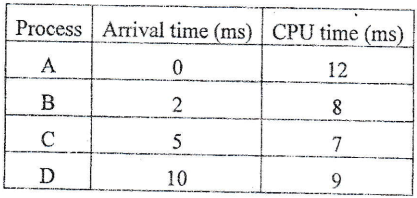
\includegraphics[width=3.5in]{os_2}
	
	\item Consider the following set of processes, with length of the CPU burst time given in milliseconds. \hspace{12.9cm} [8] (\bo{80 Ch})\\
	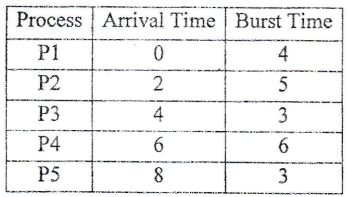
\includegraphics[width=3.5in]{os_3}\\
	With all the given information, draw the Gantt Chart and calculate the average waiting time (AWT), average turnaround time (ATAT), CPU utilization and throughput for the
	\begin{enumerate}[noitemsep, topsep = 0pt, label = \alph*.]
		\item Round Robin (RR) (Quantum Time = 2)
		\item Highest Response Ratio Next (HRRN)
	\end{enumerate}
	
	\item Make  schedule for the processes mentioned in the table below as per Shortest Remaining Time First (SRTF) algorithm. Also calculate average turnaround time and average waiting time, throughput and CPU utilization. \hfill [6] (\bo{\texttt{80 Bh}})
	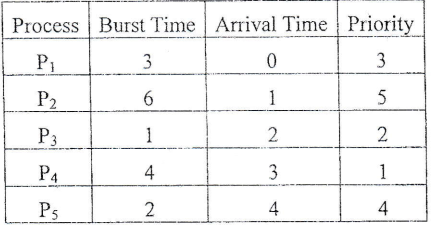
\includegraphics[width=3.5in]{os_4}
	
	\item Apply MLQ scheduling for following set of processes of two queues Q1 and Q2 where Priority of Q1 is greater than that of Q2 and Q1 uses Round Robin (Time Quantum = 2) and Q2 uses FCFS. Construct Gantt-Chart and computer average TAT for above scenario.\\ \enter \hfill [4] (\texttt{80 Ba})\\
	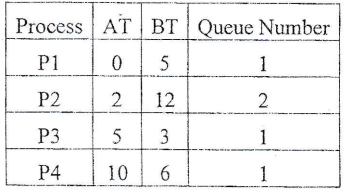
\includegraphics[width=3.5in]{os_5}
	
	\item Consider following set of process with given arrival and CPU burst time. Calculate the average waiting time for each of process for non-primitive shortest job first (SJF) and Round Robin Scheduling Algorithms with quantum size 4. \hfill [5] (\bo{79 Ch})\\
	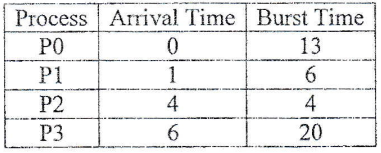
\includegraphics[width=3.5in]{os_6}
	
	\item Consider the following set of processes, with arrival time and the length of CPU burst time given in millisecond as below: \hfill [6] (76 Ba)\\
	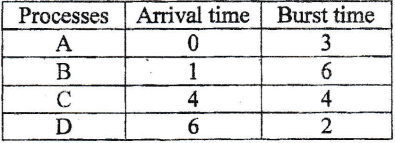
\includegraphics[width=3.5in]{os_10}\\
	\begin{enumerate}[noitemsep, topsep = 0pt, label = \alph*.]
		\item Draw Gantt chart illustrating the execution of these processes using FCFS, SRTN and RR (Quantum = 2) scheduling.
		\item What is the waiting time and Turnaround time of each process for each of th escheduling algorithm?
	\end{enumerate}
	
	\item Let us consider five process with given arrival time and length of the CPU burst given in milliseconds. Calculate the turnaround time and waiting time for all processes applying First Come First Serve, Shortest Job first and Round Robin (time quantum = 3) algorithms.\\
	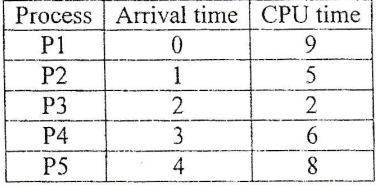
\includegraphics[width=3.5in]{os_8}
	\hfill [6] (\bo{\texttt{79 Bh}})
	
	\item Assume the process arrived in the order p\sub{1}, p\sub{2}, p\sub{3}, p\sub{4} and p\sub{5} all time 0, priority 1 as highest and 4 as lowest. \hfill [8] (\bo{78 Ch})\\
	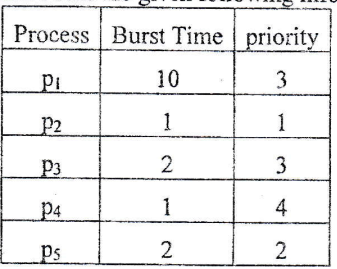
\includegraphics[width=2in]{os_7}
	\begin{enumerate}[noitemsep, topsep = 0pt, label = \alph*.]
		\item Draw the gantt chart
		\item Calculate average waiting time and average turnaround for the following scheduling algorithm.\\
		i. Round robin (quantum = 1)\\
		ii. priority preemptive\\
		iii. preemptive SJF\\
		iv. FCFS
	\end{enumerate}
	
	\item Consider the following processes, with the length of the CPU burst time in millisecond. The processes are assumed to have arrived in the order P1, P2, P3, P4, P5 all at time 0. [Lowest number being Highest Priority] \hfill [6] (\bo{75 Bh})
	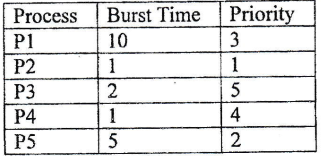
\includegraphics[width=3.5in]{os_11}\\
	Draw Gantt chart illustrating priority and RR (quantum = 1) scheduling. Also find average waiting time and average turn-around time for each of the algorithms.
	
	\item Consider the following set of processes, with arrival time and the length of CPU burst time given in millisecond as below: \hfill [4+4] (\bo{81 Bh})
	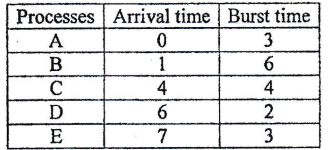
\includegraphics[width=3.5in]{os_9}
	\begin{enumerate}[noitemsep, topsep = 0pt, label = \alph*.]
		\item Draw Gantt chart illustrating the execution of these processes using FCFS, SRTN and RR (Quantum = 3) scheduling.
		\item What is the waiting time and Turnaround time of each process for each of the scheduling algorithm?
	\end{enumerate}
		
\end{enumerate}
\subsection{Multiprocessor Scheduling concept}

\pagebreak
\section{Process Communication and Synchronization}
\begin{center}(5 Hours/10 Marks)\end{center}
\subsection{Principles of Concurrency}
\subsection{Critical Region}
\subsection{Race Condition}
\subsection{Mutual Exclusion}
\subsection{Semaphores and Mutex}
\subsection{Message Passing}
\subsection{Monitors}
\subsection{Classical Problems of Synchronization: Readers-Writers Problem, Producer Consumer Problem, Dining Philosopher problem}

\pagebreak
\section{Memory Management}
\begin{center}(6 Hours/10 Marks)\end{center}
\subsection{Memory address, Swapping and Managing Free Memory Space}
\subsection{Resident Monitor}
\subsection{Multiprogramming with Fixed Partition}
\subsection{Multiprogramming With Variable Partition}
\subsection{Multiple Base Register}
\subsection{Virtual Memory Management}
\subsubsection{Paging}
\subsubsection{Segmentation}
\subsubsection{Paged Segmentation}
\subsection{Demand Paging}
\subsection{Performance}
\subsection{Page Replacement Algorithms}
\subsection{Allocation of Frames}
\subsection{Thrashing}

\pagebreak
\section{File Systems}
\begin{center}(6 Hours/10 Marks)\end{center}
\subsection{File: Name, Structure, Types, Access, Attribute, Operations}
\subsection{Directory and File Paths}
\subsection{File System Implementation}
\subsubsection{Selecting Block Size}
\subsubsection{Impact of Block Size Selection}
\subsubsection{Implementing File: Contiguous Allocation, Link List Allocation, Link List Allocation with Table, Inode}
\subsubsection{Implementing Directory}
\subsection{Impact of Allocation Policy on Fragmentation}
\subsection{Mapping File Blocks on The Disk Platter}
\subsection{File System Performance}
\subsection{Example File Systems: CD ROM file system, MS-DOS file system, Unix File system}

\pagebreak
\section{I/O Management and Disk Scheduling}
\begin{center}(4 Hours/7 Marks)\end{center}
\subsection{Principles of I/O Hardware}
\subsection{Principles of I/O software}
\subsection{I/O software Layer}
\subsection{Disk}
\subsubsection{Hardware}
\subsubsection{Formatting}
\subsubsection{Arm scheduling}
\subsubsection{Error handling}
\subsubsection{Stable Storage}

\pagebreak
\section{Deadlock}
\begin{center}(5 Hours/10 Marks)\end{center}
\subsection{Principles of deadlock}
\subsection{Deadlock Prevention}
\subsection{Deadlock Avoidance}
\subsection{Deadlock Detection}
\subsection{Recovery from deadlock}
\subsection{An Integrated Deadlock Strategies}
\subsection{Other Issues: Two phase locking, Communication Deadlock, Livelock, Starvation}

\pagebreak
\section{Security}
\begin{center}(4 Hours/7 Marks)\end{center}
\subsection{Security breaches}
\subsection{Types of Attacks}
\subsection{Security Policy and Access Control}
\subsection{Basics of Cryptography}
\subsection{Protection Mechanisms}
\subsection{Authentication}
\subsection{OS Design Considerations For Security}
\subsection{Access Control Lists And OS Support}

\pagebreak
\section{System administration}
\begin{center}(4 Hours/6 Marks)\end{center}
\subsection{Administration Tasks}
\subsection{User Account Management}
\subsection{Start And Shutdown Procedures}
\subsection{Setting up Operational Environment for a New User}
\subsection{AWK tool, Search, Sort tools, Shell scripts, Make tool}

\end{document}
